%----------------------------------------------------------------------------------------
%	PACKAGES AND THEMES
%----------------------------------------------------------------------------------------
\documentclass{beamer}
% Load a bunch of useful packages:
\usepackage{amssymb,amsmath,amsfonts,mathtools} % useful math fonts and symbols
\usepackage{geometry} % allows changing margins and sizes of stuff
\usepackage{hyperref} % allows referencing of lines of text, urls, figures etc
\usepackage{natbib} % allows citation referencing from a .bib file
\bibliographystyle{apalike} % American Psychological Association style guide
\usepackage{graphicx} % to include graphics from the figures folder with helpful formating options
\usepackage{tikz}
\usetikzlibrary{arrows}
\usepackage{pgfplots}
\usetikzlibrary{calc}
%---------------------------------------------%
\usepackage{color} % custom color definitions:%
    %UOregon colors:                          %
    \definecolor{UOGreen}{RGB}{18, 71, 52}    %
    \definecolor{UOYellow}{RGB}{254, 225, 35} %
    %Secondary official colors:               %
    \definecolor{LegacyGreen}{HTML}{104735}   %
    \definecolor{GrassGreen}{HTML}{489D46}    %
    \definecolor{LimeGreen}{HTML}{8ABB40}     %
    \definecolor{Chartreuse}{HTML}{E2E11B}    %
    \definecolor{Berry}{HTML}{8D1D58}         %
    \definecolor{DarkBlue}{HTML}{004F6E}      %
    \definecolor{LightBlue}{HTML}{00A5B5}     %
    \definecolor{crimson}{RGB}{ 170, 4, 36 }
    \definecolor{darkblue}{RGB}{ 4, 47, 170 }
    \definecolor{brown}{RGB}{ 111, 71, 2 }
    \definecolor{periwinkle}{RGB}{ 90, 177, 204 }
    \definecolor{ducksgreen}{HTML}{007030}
%----------------------------------------------

\usepackage{setspace} % to specify single, double or one-half spacing of text
\usepackage{indentfirst} % indent first line of a text paragraph
\usepackage{multicol} %multipage ability
\usepackage{multirow}
\usepackage{ulem} % \ul (underline) command which will break over line ends
\usepackage{amsthm} % allows standarized theorem commands
\setbeamertemplate{theorems}[numbered]
\theoremstyle{plain}
\newtheorem{assume}{Assumption}
\newtheorem{define}{Definition}
\usepackage{breqn} %automatic line breaking
\normalem

% Theming and Appearance Setup:
\usetheme{metropolis}
\metroset{block=fill}
%\usetheme{default}
\usefonttheme{professionalfonts}
\fontfamily{ppl}\selectfont
\usecolortheme[named=UOGreen]{structure}
\setbeamertemplate{footline}[frame number]
\setbeamertemplate{headline}{} %Removes Section Index on top of slide
\beamertemplatenavigationsymbolsempty
\hypersetup{
    colorlinks=true,
    linkcolor=DarkBlue,
    filecolor=Berry,
    citecolor=GrassGreen,
    urlcolor={LightBlue},
    pdftitle={Trade and Labor Market Dynamics},
    pdfpagemode=FullScreen
}

%------------------------------------------------------------------------------%TITLE PAGE
%------------------------------------------------------------------------------
% The title
\title{Uncertainty \& Information Topics}
\author{Dante Yasui }
\institute{EC327 Game Theory}
\date{Winter 2024}
\titlegraphic{
\includegraphics[scale=.4]{UOSignature-356.png}}


%-----------------------------------------------------------------------------
%	PRESENTATION SLIDES
%-----------------------------------------------------------------------------

\begin{document}

\begin{frame}[plain]
    % Print the title page as the first slide
    \titlepage
\end{frame}
\addtocounter{framenumber}{-1}

\begin{frame}[plain]{Outline}
  \tableofcontents
\end{frame}
\addtocounter{framenumber}{-1}

% - - - - - - - - - - - - - - - - - - - - - - - - - - - - - - - - - - - - - -

% \section{Topics and Definitions}
% 
% - - - - - - - - - - - - - - - - - - - - - - - - - - - - - - - - - - - - - - -
\begin{frame}{What is Asymmetric Info?}
  \begin{itemize}
    \item We already learned about \textit{symmetric} uncertainty
    in the models where \texttt{Nature} makes a play
    that \textit{neither} player can observe.
    \item But sometimes one player will know some things that other do not.
  \end{itemize}
  \begin{block}{Asymmetric Information}
    describes situations in which some players have \alert{private information}
    that is not accessible to other players.
  \end{block} 
\end{frame}

% - - - - - - - - - - - - - - - - - - - - - - - - - - - - - - - - - - - - - - -

\begin{frame}{What is Asymmetric Info?}
  If you are \alert{better informed} than others:
  \begin{itemize}
    \item You might be able to 
    \textit{conceal} or \textit{reveal misleading} information strategically
    in order to manipulate the beliefs of others about you 
    \item You might instead want to \textit{selectively reveal} the truth
    if it helps you.
  \end{itemize}
  If you are \alert{less informed} than other players:
  \begin{itemize}
    \item You might want to \textit{filter out the truth} from lies or misinformation.
    \item You could instead strategically \textit{remain ignorant} 
    in order to claim "credible deniability".
  \end{itemize}
\end{frame}

% - - - - - - - - - - - - - - - - - - - - - - - - - - - - - - - - - - - - - - -

\begin{frame}{Behaviors in Asymmetric Info Games}
  \begin{block}{Cheap Talk}
    I could let people in on my private info by directly talking to them.
    But if they know that I have potential incentives to \textit{lie},
    they might not believe my \alert{\textit{cheap talk}}.
  \end{block}
  \begin{quote}
    Actions Speak Louder Than Words 
  \end{quote}
\end{frame}

% - - - - - - - - - - - - - - - - - - - - - - - - - - - - - - - - - - - - - - -

\begin{frame}{Behaviors in Asymmetric Info Games}
  \begin{block}{Signaling}
    When I know something about myself 
    that would benefit me if \textit{others} knew,
    I might send a \alert{signal} through my actions
  \end{block}
  Examples:
  \begin{itemize}
    \item
    A 4.0 GPA might signal to potential employers that you are hard-working.
    \item
    If you're in the market for a product and you're uncertain of its quality,
    a money-back guarantee might \textit{signal} that it works.
  \end{itemize}
\end{frame}

% - - - - - - - - - - - - - - - - - - - - - - - - - - - - - - - - - - - - - - -

\begin{frame}{Behaviors in Asymmetric Info Games}
  \begin{block}{Screening}
    When I want to know something about \textit{someone else's} private info,
    I might get them to take an action that would \alert{screen} out 
    people of different \textit{types}.
  \end{block}
  Examples:
  \begin{itemize}
    \item 
    An employer might not know if a job candidate is a \textit{lazy}
    or \textit{industrious} type of worker,
    but they could try to screen out the \textit{lazy} ones
    by requiring a portfolio of previous work.
  \end{itemize}
\end{frame}

% - - - - - - - - - - - - - - - - - - - - - - - - - - - - - - - - - - - - - - -

\begin{frame}{Effectiveness of Different Communication Strategies}
  When are different strategies effective in actually revealing private info?
  \begin{itemize}
    \item 
    Sometimes direct communication works when players' interests align.
    But trust might break down when there are incentives to send false messages.
    \item 
    A signal is only effective if not all types take the same action.
    We'll discuss breakdowns in signaling using the ideas of 
    \alert{Separating} vs \alert{Pooling} equilibria
  \end{itemize}
\end{frame}

% - - - - - - - - - - - - - - - - - - - - - - - - - - - - - - - - - - - - - - -

\begin{frame}{Asymmetric Info in Market Games}
  \begin{itemize}
    \item 
    In 201 or 311 you may have learned about the 
    \textbf{perfectly competitive} markets model. \\
    \item 
    One of the assumptions of that model is \alert{perfect information}. \\ 
    \item 
    When this assumption breaks, we might see \alert{Adverse Selection}
    or other types of market failures.
\end{itemize}
\end{frame}

% 
% \section{Cheap Talk}
% 
% - - - - - - - - - - - - - - - - - - - - - - - - - - - - - - - - - - - - - - -

\begin{frame}{Cheap Talk Equilibrium - When Interests Align}
  Suppose that I want to meet up with Jose at a coffee shop on campus.
  \begin{table}[!h]
    \centering
    \begin{tabular}{cc|c|c|}
    & \multicolumn{1}{c}{} & \multicolumn{2}{c}{Jose}\\
    & \multicolumn{1}{c}{} & \multicolumn{1}{c}{$Starbucks$}  & \multicolumn{1}{c}{$Roma$} \\\cline{3-4}
    \multirow{2}*{Dante}  & $Starbucks$ & $1, 1$ & $0,0$ \\\cline{3-4}
                          & $Roma$       & $0, 0$ & $2,2$ \\\cline{3-4}
  \end{tabular}
  \end{table}

  We'll also add a first stage to this game 
  where Dante can send Jose a text message saying either 
  \textit{"I'm going to Starbucks"} or \textit{"I'm going to Roma"}.
\end{frame}

% - - - - - - - - - - - - - - - - - - - - - - - - - - - - - - - - - - - - - - -

\begin{frame}{Cheap Talk Equilibria - When Interests Align}
  The strategy profile where:
  \begin{itemize}
    \item  
    I send the message \textit{"going to Starbucks"}
    \item
    we both go to Starbucks if I send \textit{"going to Starbucks"}
    \item 
    or both go to Roma if I send \textit{"going to Roma"}
  \end{itemize}
  is a \textbf{Nash Equilibrium} (specifically a \textit{subgame perfect} NE).
  \begin{itemize}
    \item We'll call this a \alert{"cheap talk"} equilibrium 
    because it was in my best interest to communicate my actual strategy.
    \item It cost me nothing to send a \textit{message}.
  \end{itemize}
\end{frame}

% - - - - - - - - - - - - - - - - - - - - - - - - - - - - - - - - - - - - - - -

\begin{frame}{Cheap Talk vs Babbling Equilibrium}
  However, this is not the only SPNE of this game.
  If are strategy profiles in the second stage are:
  \begin{itemize}
    \item 
    Jose will go to Starbucks no matter what message Dante sends
    \item
    Dante will go to Starbucks no matter what message he sent
  \end{itemize}
  Then Dante will be indifferent between sending either message in the first place.

  \begin{itemize}
    \item 
    We'll call this a \alert{"babbling" equilibrium} 
    because the initial message sends \textit{no} information about what 
    I will actually do.
    \item 
    This equilibrium seems unlikely, but if I have an existing \textit{reputation}
    for always going to Starbucks, this would be plausible 
    and completely rational behavior.
  \end{itemize}
\end{frame}

% - - - - - - - - - - - - - - - - - - - - - - - - - - - - - - - - - - - - - - -

\begin{frame}{Cheap Talk Equilibria - When Interests are Conflicting}
  What about a zero-sum game?
  \begin{table}[!h]
    \centering
    \begin{tabular}{cc|c|c|}
    & \multicolumn{1}{c}{} & \multicolumn{2}{c}{Navratilova}\\
    & \multicolumn{1}{c}{} & \multicolumn{1}{c}{$DL$}  & \multicolumn{1}{c}{$CC$} \\\cline{3-4}
    \multirow{2}*{Evert}  & $DL$ & $50, 50$ & $80,20$ \\\cline{3-4}
                          & $CC$ & $90, 10$ & $20,80$ \\\cline{3-4}
  \end{tabular}
  \end{table}
  \begin{itemize}
    \item  
    Should Navratilova believe what Evert says she will do?
    \item 
    Should Navratilova believe that Evert will do 
    \textit{exactly the opposite} of what she says she'll do?
  \end{itemize}
\end{frame}

% - - - - - - - - - - - - - - - - - - - - - - - - - - - - - - - - - - - - - - -

\begin{frame}{Cheap Talk Equilibria - When Interests are Conflicting}
  What about a zero-sum game?
  \begin{table}[!h]
    \centering
    \begin{tabular}{cc|c|c|}
    & \multicolumn{1}{c}{} & \multicolumn{2}{c}{Navratilova}\\
    & \multicolumn{1}{c}{} & \multicolumn{1}{c}{$DL$}  & \multicolumn{1}{c}{$CC$} \\\cline{3-4}
    \multirow{2}*{Evert}  & $DL$ & $50, 50$ & $80,20$ \\\cline{3-4}
                          & $CC$ & $90, 10$ & $20,80$ \\\cline{3-4}
  \end{tabular}
  \end{table}
  \begin{itemize}
    \item 
    The only equilibrium of this game is a \alert{babbling} equilibrium.
    \item 
    There is no message that Evert could send
    that would give Navratilova any more idea of what she will actually play.
  \end{itemize}
\end{frame}

% - - - - - - - - - - - - - - - - - - - - - - - - - - - - - - - - - - - - - - -

\begin{frame}{Cheap Talk Equilibria - Partially Aligned Interests}
  Many real life games have mixtures of conflict and common interest.
  \begin{itemize}
    \item 
    The question of whether direct communication is \textit{credible} or not 
    will depend on the relative degree of each incentive.
    \item 
    We will use our tools from the first half of the course 
    to make testable predictions based on different ranges of assumptions.
  \end{itemize}
\end{frame}

% - - - - - - - - - - - - - - - - - - - - - - - - - - - - - - - - - - - - - - -

\begin{frame}{Defensive Medicine}
  \begin{quote}
    In a recent survey of physicians,
    93\% reported altering their clinical behavior 
    because of the threat of malpractice liability.
    Of them, 92\% used “assurance behavior” 
    such as ordering tests, performing diagnostic procedures,
    and referring patients for consultation;
    and 43\% reported using imaging technology 
    in clinically unnecessary circumstances. 
  \end{quote}  
  Harrington, pg. 461
\end{frame}

% - - - - - - - - - - - - - - - - - - - - - - - - - - - - - - - - - - - - - - -

\begin{frame}{Defensive Medicine}
  \begin{itemize}
    \item 
    Consider a patient who goes to the doctor for an examination. 
    \item
    The doctor can recommend an expensive test
    that is not fully covered by the patient's insurance.
    \item 
    The doctor cares about the patient, 
    but also doesn't want to be sued for malpractice 
    if the patient \textit{does} end up needing the test 
    and the doctor didn't recommend it.
    \item 
    The patients value $v$ from a beneficial test is 5,
    and $v=-5$ if the test is useless.
    \item 
    We'll use $a$ to stand in for the value of a test to a doctor 
    from a malpractice standpoint.
  \end{itemize}
\end{frame}

% - - - - - - - - - - - - - - - - - - - - - - - - - - - - - - - - - - - - - - -

\begin{frame}{Defensive Medicine}
  \begin{center}
    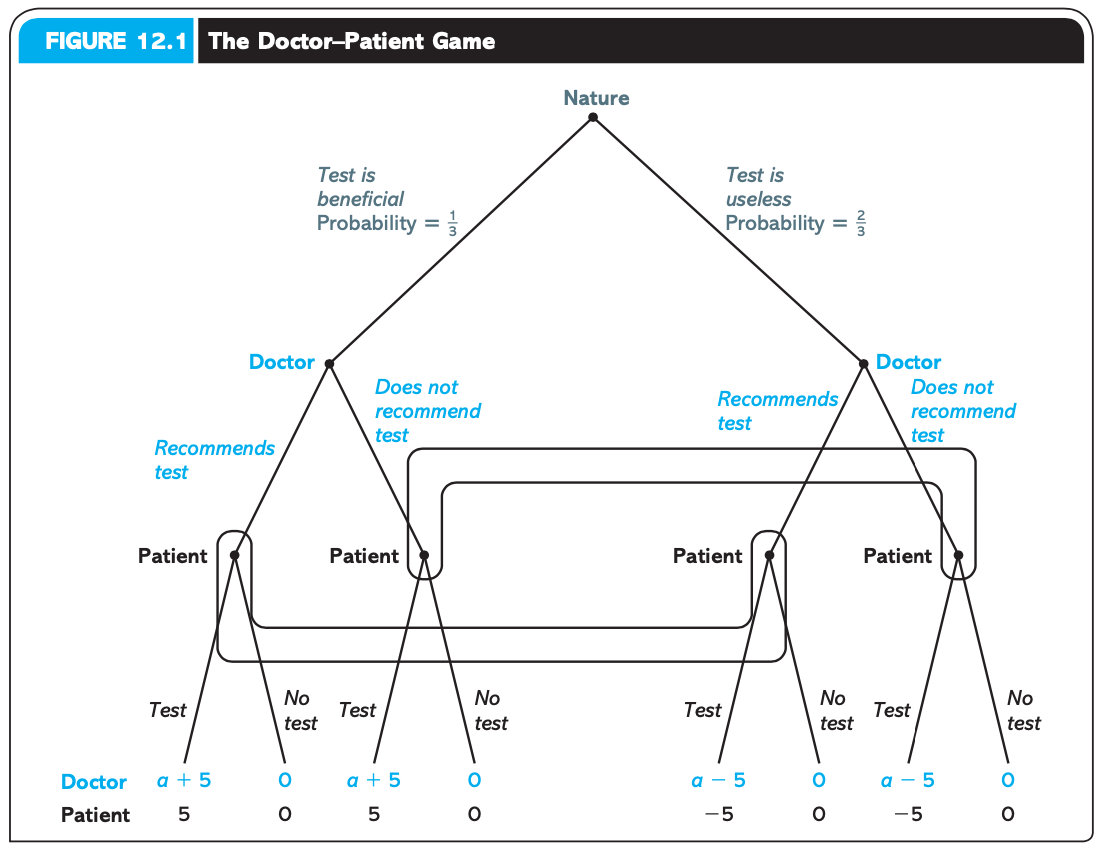
\includegraphics[width=.9\textwidth]{figures/defensivemed.png}  
  \end{center} 
\end{frame}

% - - - - - - - - - - - - - - - - - - - - - - - - - - - - - - - - - - - - - - -

\begin{frame}{Defensive Medicine - Babbling Strategy}
  % Why is defensive medicine so pervasive?
  \begin{block}{Pooling Equilibrium}
    \begin{itemize}
      \item \underline{Doctor's Strategy:}
      Recommend the test whether or not it is beneficial.
      \item \underline{Patient's Strategy:}
      Ignore the doctor's recommendation.
      \item \underline{Patient's Beliefs:}
      Ignoring the doctors advice,
      the probability the test is effective is 1/3.
    \end{itemize} 
  \end{block}
  \begin{itemize}
    \item This equilibrium is a \textit{babbling equilibrium}.
    \item The doctor's recommendation contains no real signal to the patient.
  \end{itemize}
\end{frame}

% - - - - - - - - - - - - - - - - - - - - - - - - - - - - - - - - - - - - - - -

\begin{frame}{Defensive Medicine - Babbling Strategy}
  % Why is defensive medicine so pervasive?
  \begin{block}{Pooling Equilibrium}
    \begin{itemize}
      \item \underline{Doctor's Strategy:}
      Recommend the test whether or not it is beneficial.
      \item \underline{Patient's Strategy:}
      Ignore the doctor's recommendation.
      \item \underline{Patient's Beliefs:}
      Ignoring the doctors advice,
      the probability the test is effective is 1/3.
    \end{itemize} 
  \end{block}
  \begin{itemize}
    \item The patient's beliefs are consistent, 
    and their expected utility from taking the test
    is $\frac{1}{3} \cdot 5 + \frac{2}{3} \cdot (-5) = - \frac{5}{3}$.
    \item Given that the patient will never take the test, 
    the doctor is indifferent between recommending the test or not.
    \item So this situation in which the doctor always recommends the test
    and the patient always ignores their advice is \textit{stable}.
  \end{itemize}
\end{frame}

% - - - - - - - - - - - - - - - - - - - - - - - - - - - - - - - - - - - - - - -

\begin{frame}{Defensive Medicine - Separating Strategies}
  The previous result was disappointing, but not unexpected.
  \begin{block}{Insight}
    For every cheap talk game, there is always a babbling equilibrium.
  \end{block}
  \begin{itemize}
    \item But let's now focus on the more interesting question
    of how to make the doctor's recommendation \textit{meaningful}.
  \end{itemize}
\end{frame}

% - - - - - - - - - - - - - - - - - - - - - - - - - - - - - - - - - - - - - - -

\begin{frame}{Defensive Medicine - Separating Strategies}
  Consider the following strategy profile:
  \begin{block}{}
    \begin{itemize}
      \item \underline{Doctor's Strategy:}
      Recommend the test if and only if it is beneficial.
      \item \underline{Patient's Strategy:}
      Follow the doctor's recommendation.
      \item \underline{Patient's Beliefs:}
      \begin{itemize}
        \item If the doctor recommends the test,
        then the test is beneficial with 100\% probability.
        \item If the doctor does not recommend the test,
        then the test is beneficial with 0\% probability.
      \end{itemize}
    \end{itemize}
  \end{block}
\end{frame}

% - - - - - - - - - - - - - - - - - - - - - - - - - - - - - - - - - - - - - - -

\begin{frame}{Defensive Medicine - Separating Strategies}
  When will the doctor follow the separating strategy?
  \begin{enumerate}
    \item When 
    $EU_d(\text{Rec. when beneficial}, (T,NT)) 
    \geq EU_d(\text{Don't rec. when beneficial}, (T,NT))$ 
    \vspace{12mm}
    \item and when 
    $EU_d(\text{Don't rec. when useless}, (T,NT)) 
    \geq EU_d(\text{Rec. when useless}, (T,NT))$ 
    \vspace{12mm}
  \end{enumerate}
  Solve for the range of $a$ where this is a NE.  
\end{frame}

% - - - - - - - - - - - - - - - - - - - - - - - - - - - - - - - - - - - - - - -


\begin{frame}{Defensive Medicine - Separating Strategies}
  When will the doctor follow the separating strategy?
  \begin{enumerate}
    \item When 
    $EU_d(\text{Rec. when beneficial}, (T,NT)) 
    \geq EU_d(\text{Don't rec. when beneficial}, (T,NT))$ 
    $$ a + 5 \geq 0 $$
    \item and when 
    $EU_d(\text{Don't rec. when useless}, (T,NT)) 
    \geq EU_d(\text{Rec. when useless}, (T,NT))$ 
    $$ 0 \geq a - 5 \Rightarrow a \leq 5 $$
  \end{enumerate}
  Solve for the range of $a$ where this is a NE.  
  $$ -5 \leq a \leq 5 $$
\end{frame}

% - - - - - - - - - - - - - - - - - - - - - - - - - - - - - - - - - - - - - - -
\begin{frame}{Defensive Medicine - Conclusions}
  Interpreting our findings:
  \begin{itemize}
    \item 
    When $a=0$, the doctor's interests are \textit{perfectly} aligned 
    with the patient's.
    \item 
    When $a\leq5$, the doctor's interests are \textit{partially} aligned 
    with the patient's interests,
    and there is an equilibrium where the doctor gives truthful recommendations.
    \item 
    When $a>5$, there is only a babbling equilibrium
    because the doctor's incentives are to not be truthful.
    Even if they did give a truthful recommendation,
    the patient would have no reason to believe it would be \textit{credible}.
  \end{itemize}
\end{frame}

% - - - - - - - - - - - - - - - - - - - - - - - - - - - - - - - - - - - - - - -

\begin{frame}{Defensive Medicine - Conclusions}
  Connecting with our real-world observations:
  \begin{itemize}
    \item 
    We don't know what doctors' subjective costs of malpractice threats are
    ($a$).
    \item 
    But we can observe their \textit{behaviors}.
    \item 
    If we see that doctors recommend more tests than are beneficial,
    it might reveal that $a$ is quite large. 
  \end{itemize}
  \begin{block}{Revealed Preference}
    The idea that people reveal their true preferences by the choices they make.
  \end{block}
\end{frame}





% 
% \section{Adverse Selection}
% 
\begin{frame}{Adverse Selection - Definition}
  \begin{block}{Adverse Selection}
  When one player knows something about the outcomes that others don't 
  and direct communication will not \textit{credibly} signal their information,
  there can be separating equilibria in which only those players
  with the 'undesirable' states of information will 
  self-\textit{select} into engaging in the market.
  \end{block}
\end{frame}

% - - - - - - - - - - - - - - - - - - - - - - - - - - - - - - - - - - - - - - -

\begin{frame}{Adverse Selection - Examples}
  \underline{\Large{Insurance Markets}}
  \begin{itemize}
    \item Potential buyers of insurance have different risk levels
    that they know about themselves but are not easily (or legally)
    observable to insurance plan providers.
    \begin{itemize}
      \item Underlying health conditions, riskier driving habits, etc.
    \end{itemize}
    \item Insurance providers have to pay out more often
    on these riskier customers.
    \item However, riskier customers are the exact types 
    who will find insurance plans more attractive.
  \end{itemize}
\end{frame}

% - - - - - - - - - - - - - - - - - - - - - - - - - - - - - - - - - - - - - - -

\begin{frame}{Adverse Selection - Examples}
  \underline{\Large{Insurance Markets}}
  \begin{itemize}
    \item What strategies could an insurance provider take 
    to \textit{screen} out risky customers from safe customers?
    \item Any ideas?
  \end{itemize}
\end{frame}

% - - - - - - - - - - - - - - - - - - - - - - - - - - - - - - - - - - - - - - -

\begin{frame}{Adverse Selection - Examples}
  \underline{\Large{Insurance Markets}}
  \begin{itemize}
    \item Suppose there are only two categories of risk level.
    \item An insurance provider could offer two different plans:
    \begin{itemize}
      \item Plan 1: has a lower premium
      but covers a lower percent of the customer's loss.
      \item Plan 2: has a higher premium 
      but covers a higher percent of the loss.
    \end{itemize}
  \end{itemize}
\end{frame}

% - - - - - - - - - - - - - - - - - - - - - - - - - - - - - - - - - - - - - - 

\begin{frame}{Adverse Selection - Examples}
  \underline{\Large{Insurance Markets}}
  \begin{itemize}
    \item How should the insurance provider structure the two plans 
    so that a \textit{separating equilibrium} is achieved 
    in which all risky types choose a different plan than the safe types?
    \begin{itemize}
      \item Make Plan 2 only attractive to safe types by setting the price higher than the risky types' willingness to pay for the extra security.
      \item and Plan 2 a better option for safe types than Plan 1.
      \begin{itemize}
        \item We call this \alert{incentive compatible}.
      \end{itemize}
      \item Make Plan 1 a better option for risky types than going without insturance altogether
      \begin{itemize}
        \item We call this \alert{individually rational}.
      \end{itemize}
    \end{itemize}
  \end{itemize}
\end{frame}

% - - - - - - - - - - - - - - - - - - - - - - - - - - - - - - - - - - - - - - -

\begin{frame}{Adverse Selection - Market for Lemons}
  In economics, one of the most famous examples of adverse selection 
  comes from George Akerlof's 1970 paper, 
  "The Market for Lemons: Qualitative Uncertainty and the Market Mechanism".
  \begin{itemize}
    \item He analyses the used car market, 
    in which crappy cars are called 'lemons'
  \end{itemize}
\end{frame}

% - - - - - - - - - - - - - - - - - - - - - - - - - - - - - - - - - - - - - - -

\begin{frame}{Adverse Selection - Market for Lemons}
  \begin{itemize}
    \item Suppose there are only two types of cars:
    \begin{itemize}
      \item good quality cars are valued at \$12,500 to the seller
      \item and lemons are worth \$3,000. 
    \end{itemize}
    \item Suppose a potential buyer would be willing to pay more than these values. 
    \begin{itemize}
      \item He would be willing to pay \$16,000 for a car he knows is good
      \item and \$6,000 for a car he knows is a lemon.
    \end{itemize}
  \end{itemize}
\end{frame}

% - - - - - - - - - - - - - - - - - - - - - - - - - - - - - - - - - - - - - - -

\begin{frame}{Adverse Selection - Market for Lemons}
  In a perfectly competitive market with perfect info
  and a large number of buyers:
  \begin{itemize}
    \item buyer competition will drive up prices to 
    \$16,000 for good cars and \$6,000 for lemons.
  \end{itemize}
\end{frame}

% - - - - - - - - - - - - - - - - - - - - - - - - - - - - - - - - - - - - - - -

\begin{frame}{Adverse Selection - Market for Lemons}
  However, buyers don't know the true value of any car by looking at them,
  but the seller knows whether their car is a lemon or not.
  \begin{itemize}
    \item Now we have a market with \alert{aymmetric info}
    \item When the type of car is unobservable,
    there can only be \textit{one price} in the market
  \end{itemize}
\end{frame}

% - - - - - - - - - - - - - - - - - - - - - - - - - - - - - - - - - - - - - - -

\begin{frame}{Adverse Selection - Market for Lemons}
   Suppose that a fraction $f$ of cars are 'oranges' \\ 
   and the remaining $(1-f)$ fraction are 'lemons' \\
   Draw the extensive form game tree
\end{frame}

% - - - - - - - - - - - - - - - - - - - - - - - - - - - - - - - - - - - - - - -

\begin{frame}{Market for Lemons - Buyer's Perspective}
  For the buyer: \\ 
  write out the expected utility of buying a car at price $p$:
  \pause
  $$16000\cdot f + 6000 \cdot (1-f)$$
  \begin{itemize}
    \item For what price will a buyer be willing to buy a car of unknown quality?
    \pause
    $$p \leq 16000 + 10000\cdot f$$
  \end{itemize}
\end{frame}

% - - - - - - - - - - - - - - - - - - - - - - - - - - - - - - - - - - - - - - -

\begin{frame}{Market for Lemons - Seller's Perspective}
  For the seller: \\ 
  \begin{itemize}
    \item What price $p$ would make the owner of a lemon willing to sell?
      \pause
      \begin{itemize}
        \item \$3000
      \end{itemize}
    \item What price would make the owner of an organge willing to sell?
      \pause
      \begin{itemize}
        \item \$12500
      \end{itemize}
  \end{itemize}
\end{frame}

% - - - - - - - - - - - - - - - - - - - - - - - - - - - - - - - - - - - - - - -

\begin{frame}{Market for Lemons - Market Clearing}
  When will all buyers and sellers want to trade?
  \pause
  $$12500 \leq p \leq 6000 + 10000f$$
\end{frame}

% - - - - - - - - - - - - - - - - - - - - - - - - - - - - - - - - - - - - - - -

\begin{frame}{Market for Lemons - Market Unraveling}
  When will there be a \textit{separating equilibrium}
  where only one type of car is sold?
  \pause
  $$f < 0.65$$
  \pause
  What type of car is sold in this equilibrium?
  \begin{itemize}
    \item Only \textbf{lemons}!
  \end{itemize}
\end{frame}

% - - - - - - - - - - - - - - - - - - - - - - - - - - - - - - - - - - - - - - -

\begin{frame}{Market for Lemons - Market Unraveling}
  When will there be a \textit{pooling equilibrium}
  where \textit{all} types of car are sold?
  \pause
  $$f > 0.65$$
  \pause
\end{frame}

% - - - - - - - - - - - - - - - - - - - - - - - - - - - - - - - - - - - - - - -

\begin{frame}{Market for Lemons - Conclusions}
  \begin{quote}
    \small{
    "Verbal declarations are costless and therefore useless. Anyone can lie about why he is selling the car. 
    One can offer to let the buyer have the car checked. The lemon owner can make the same offer. It’s a bluff. If called, nothing is lost. Besides, such checks are costly. \\
    Reliability reports from the owner’s mechanic are untrustworthy. The clever nonlemon owner might pay for the checkup but let the purchaser choose the inspector. The problem for the owner, then, is to keep the inspection cost down. 
    Guarantees do not work. The seller may move to Cleveland, leaving no forwarding address." 
    }
  \end{quote} 
   \footnotesize{- A. Michael Spence, \textit{Market Signaling: Information Transfer in Hiring and Related Screening Processes}}
\end{frame}

% - - - - - - - - - - - - - - - - - - - - - - - - - - - - - - - - - - - - - - -

\begin{frame}{Market for Lemons - Discussion}
  \begin{itemize}
  \item How well do you think that the used car market in the real world  
  reflects the Market for Lemons model?
  \item What other factors could there be that allow used car sellers 
  to \textit{credibly signal} the quality of their cars?
  \end{itemize}
\end{frame}

% 
% \section{Risk Preferences}
% \begin{frame}{Imperfect Info: Dealing with Risk}
  Some of you have already started asking 
  about whether different \alert{preferences for risk} might change the solutions 
  to some of the games we have looked at. 
  \begin{itemize}
    \item So far, I have abstracted away from these questions 
    by saying that we should take the payoffs given 
    as the agents' \textit{true subjective utilities}.
    \item But we can also use the tools of \textbf{utility functions}
    we introduced in the beginning of the class 
    to more explicitly model risk preferences.
  \end{itemize}
\end{frame}

% - - - - - - - - - - - - - - - - - - - - - - - - - - - - - - - - - - - - - - -

\begin{frame}{Playing with Chance}
  To review, suppose that Nature plays probabilistically with 50:50 odds:
  \begin{center}
    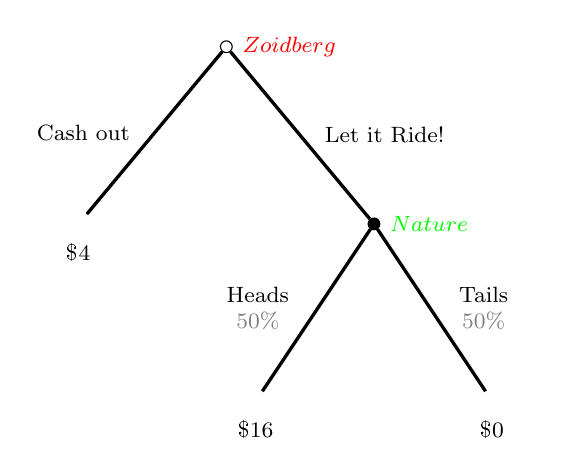
\begin{tikzpicture}[scale=1.5,font=\footnotesize, edge from parent/.style={draw, very thick}]
      \tikzstyle{solid node}=[circle,draw,inner sep=1.5,fill=black]
      \tikzstyle{hollow node}=[circle,draw,inner sep=1.5]
      \tikzstyle{level 1}=[level distance=15mm,sibling distance=2.5cm]
      \tikzstyle{level 2}=[level distance=15mm,sibling distance=2.0cm]
      \tikzstyle{level 3}=[level distance=15mm,sibling distance=1cm]
      
      \node(0)[hollow node,label=right:{\color{red} $Zoidberg$}]{}
          child{node(1)[label=below:{\$$4$}]{}
              edge from parent node[left,xshift=-5]{Cash out}
          }
          child{node(2)[solid node,label=right:{\color{green}$Nature$}]{}
              child{node[label=below:{\$$16$}]{} edge from parent node[left]{
              \begin{tabular}{c}
                   Heads \\
                   {\color{gray} $50\%$} \\
              \end{tabular}
              }}
              child{node[label=below:{\$$0$}]{} edge from parent node[right]{
              \begin{tabular}{c}
                   Tails \\
                   {\color{gray} $50\%$} \\
              \end{tabular}
              }}
              edge from parent node[right,xshift=5]{Let it Ride!}
          };
    \end{tikzpicture}
  \end{center}
  What is Zoidberg's \textbf{expected value} of \textit{Let it Ride}?
\end{frame}

% - - - - - - - - - - - - - - - - - - - - - - - - - - - - - - - - - - - - - - -

\begin{frame}{Playing with Chance}
  What if the coin is \textit{unfair}?
  \begin{center}
    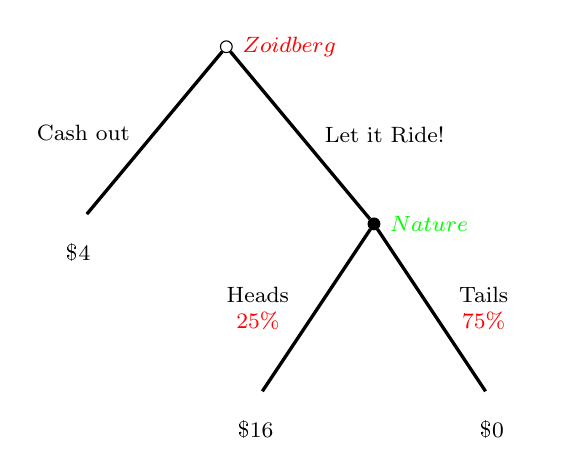
\begin{tikzpicture}[scale=1.5,font=\footnotesize, edge from parent/.style={draw, very thick}]
      \tikzstyle{solid node}=[circle,draw,inner sep=1.5,fill=black]
      \tikzstyle{hollow node}=[circle,draw,inner sep=1.5]
      \tikzstyle{level 1}=[level distance=15mm,sibling distance=2.5cm]
      \tikzstyle{level 2}=[level distance=15mm,sibling distance=2.0cm]
      \tikzstyle{level 3}=[level distance=15mm,sibling distance=1cm]
      
      \node(0)[hollow node,label=right:{\color{red} $Zoidberg$}]{}
          child{node(1)[label=below:{\$$4$}]{}
              edge from parent node[left,xshift=-5]{Cash out}
          }
          child{node(2)[solid node,label=right:{\color{green}$Nature$}]{}
              child{node[label=below:{\$$16$}]{} edge from parent node[left]{
              \begin{tabular}{c}
                   Heads \\
                   {\color{red} $25\%$} \\
              \end{tabular}
              }}
              child{node[label=below:{\$$0$}]{} edge from parent node[right]{
              \begin{tabular}{c}
                   Tails \\
                   {\color{red} $75\%$} \\
              \end{tabular}
              }}
              edge from parent node[right,xshift=5]{Let it Ride!}
          };
    \end{tikzpicture}
  \end{center}  
  What is the \textbf{expected value} now? \\ 
  Should {\color{red} Zoidberg} take the gamble?
\end{frame}

% - - - - - - - - - - - - - - - - - - - - - - - - - - - - - - - - - - - - - - -

\begin{frame}{Risk Preferences}
  Is \textbf{expected value} always the same as \alert{expected utility}?
  \begin{itemize}
    \item Suppose that I offered you a different gamble:
    \begin{itemize}
      \item \textbf{Option 1:} You get \$1,000,000 with 50\% chance,
      \$0 with 50\% chance.
      \item \textbf{Option 2:} You get \$400,000 for certain.
    \end{itemize}
    \item Which would you choose?
  \end{itemize}
\end{frame}

% - - - - - - - - - - - - - - - - - - - - - - - - - - - - - - - - - - - - - - -

\begin{frame}{Risk Preferences}
  Why would I prefer \textbf{Option 2} when it gives a lower \textit{expected payout}? 
  \begin{itemize}
    \item \$400,000 is still a life changing amount of money, 
    \item but my \alert{marginal benefit} from going from \$400,000 to \$1,000,000 
    is less than my \alert{marginal benefit} from going from \$0 to \$400,000.
    \item The \textbf{risk} of going home empty handed isn't worth the 
    payout that is a marginally larger life-changing amount of money.
  \end{itemize}
\end{frame}

% - - - - - - - - - - - - - - - - - - - - - - - - - - - - - - - - - - - - - - -

\begin{frame}{Risk Preference: Risk Aversion}
  What would a utility function with \alert{diminishing marginal benefit} 
  look like?
  \vspace{50mm}
\end{frame}

% - - - - - - - - - - - - - - - - - - - - - - - - - - - - - - - - - - - - - - -

\begin{frame}{Playing with Chance: Risk Averse Utility}
  Now suppose that {\color{red} Zoidberg}'s utility is 
  ${\color{red} U_{Z}(\$x) = \sqrt{x}}$
  \begin{center}
    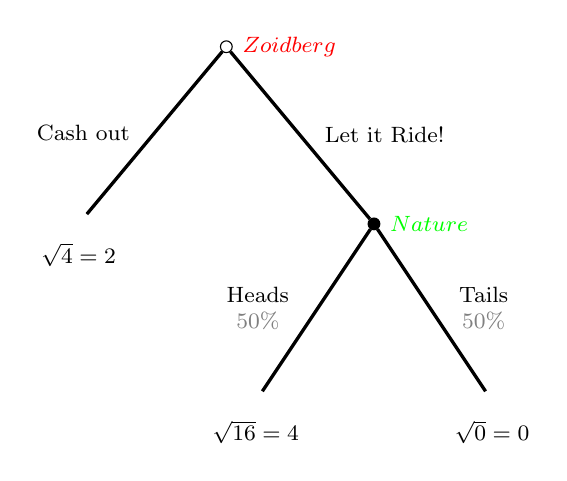
\begin{tikzpicture}[scale=1.5,font=\footnotesize, edge from parent/.style={draw, very thick}]
      \tikzstyle{solid node}=[circle,draw,inner sep=1.5,fill=black]
      \tikzstyle{hollow node}=[circle,draw,inner sep=1.5]
      \tikzstyle{level 1}=[level distance=15mm,sibling distance=2.5cm]
      \tikzstyle{level 2}=[level distance=15mm,sibling distance=2.0cm]
      \tikzstyle{level 3}=[level distance=15mm,sibling distance=1cm]
      
      \node(0)[hollow node,label=right:{\color{red} $Zoidberg$}]{}
          child{node(1)[label=below:{$\sqrt{4} = 2 $ }]{}
              edge from parent node[left,xshift=-5]{Cash out}
          }
          child{node(2)[solid node,label=right:{\color{green}$Nature$}]{}
              child{node[label=below:{$\sqrt{16} = 4$}]{} edge from parent node[left]{
              \begin{tabular}{c}
                   Heads \\
                {\color{gray} $ 50\% $}
              \end{tabular}
              }}
              child{node[label=below:{$\sqrt{0} = 0$}]{} edge from parent node[right]{
              \begin{tabular}{c}
                   Tails \\
                   {\color{gray} $ 50\% $} \\
              \end{tabular}
              }}
              edge from parent node[right,xshift=5]{Let it Ride!}
          };
    \end{tikzpicture}
  \end{center}  
  Would {\color{red} Zoidberg} be willing to cash out?
\end{frame}

% - - - - - - - - - - - - - - - - - - - - - - - - - - - - - - - - - - - - - - -

\begin{frame}{Risk Preference: Risk Seeking}
  What would a utility function with \alert{increasing marginal benefit} 
  look like?
  \vspace{50mm}
\end{frame}

% - - - - - - - - - - - - - - - - - - - - - - - - - - - - - - - - - - - - - - -

\begin{frame}{Playing with Chance: Risk Seeking Utility}
  Now suppose that {\color{blue} Bender}'s utility is 
  ${\color{blue} U_{B}(\$x) = x^2}$
  \begin{center}
    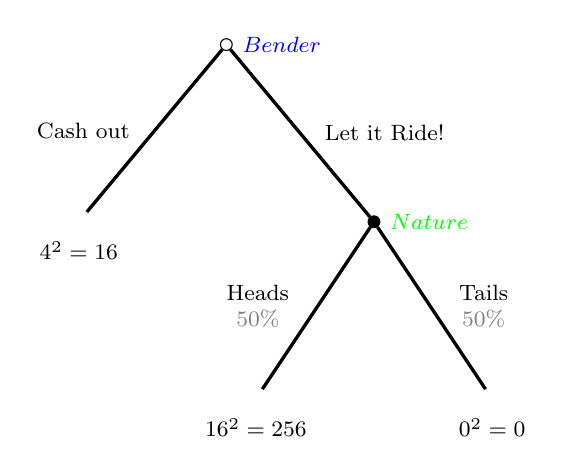
\begin{tikzpicture}[scale=1.5,font=\footnotesize, edge from parent/.style={draw, very thick}]
      \tikzstyle{solid node}=[circle,draw,inner sep=1.5,fill=black]
      \tikzstyle{hollow node}=[circle,draw,inner sep=1.5]
      \tikzstyle{level 1}=[level distance=15mm,sibling distance=2.5cm]
      \tikzstyle{level 2}=[level distance=15mm,sibling distance=2.0cm]
      \tikzstyle{level 3}=[level distance=15mm,sibling distance=1cm]
      
      \node(0)[hollow node,label=right:{\color{blue} $Bender$}]{}
          child{node(1)[label=below:{$4^2 = 16 $ }]{}
              edge from parent node[left,xshift=-5]{Cash out}
          }
          child{node(2)[solid node,label=right:{\color{green}$Nature$}]{}
              child{node[label=below:{$16^2 = 256$}]{} edge from parent node[left]{
              \begin{tabular}{c}
                   Heads \\
                {\color{gray} $ 50\% $}
              \end{tabular}
              }}
              child{node[label=below:{$0^2 = 0$}]{} edge from parent node[right]{
              \begin{tabular}{c}
                   Tails \\
                   {\color{gray} $ 50\% $} \\
              \end{tabular}
              }}
              edge from parent node[right,xshift=5]{Let it Ride!}
          };
    \end{tikzpicture}
  \end{center}  
  Would {\color{blue} Bender} be willing to cash out?
\end{frame}

% - - - - - - - - - - - - - - - - - - - - - - - - - - - - - - - - - - - - - - -

\begin{frame}{Measuring Risk Preferences}
  Both utility functions are \textbf{rational}, 
  but lead to much different behavior. \\
  How can we tell whether someone is 
  \alert{risk averse} or \alert{risk seeking}?
  \pause 
  \begin{itemize}
    \item look at their \alert{revealed preferences} 
    through the choices they make.
  \end{itemize}
\end{frame}

% - - - - - - - - - - - - - - - - - - - - - - - - - - - - - - - - - - - - - - -

\begin{frame}{Measuring Risk Preferences - Certainty Equivalent}
  \begin{itemize}
    \item Suppose that you don't know my risk preference 
    \item but you can offer me a choice between: 
    \begin{itemize}
      \item A \textbf{lottery} $L$ between \$$A$ and \$$B$ with probability $p$
      \item or a \textbf{certain} amount \$$x$ of your choosing. 
    \end{itemize}
    \item The certain amount $x$ that would make me \textit{indifferent}
    between the lottery and taking the sure payment 
    is called the \alert{certainty equivalent} of $L$.
  \end{itemize}
\end{frame}

% - - - - - - - - - - - - - - - - - - - - - - - - - - - - - - - - - - - - - - -

\begin{frame}{Measuring Risk Preferences - Certainty Equivalent}
  \begin{itemize}
    \item If my \textbf{certainty equivalent} 
    is less than the expected value of the lottery 
    \begin{itemize}
      \item you know that I am \alert{risk averse} 
    \end{itemize}
    \item If the \textbf{certainty equivalent} $>$ \textbf{$\mathbb{E}[L]$} 
    \begin{itemize}
      \item I am \alert{risk seeking}
    \end{itemize}
    \item If the \textbf{certainty equivalent} $=$ \textbf{$\mathbb{E}[L]$}
    \begin{itemize}
      \item I am \alert{risk neutral} 
    \end{itemize}
  \end{itemize} 
\end{frame}


\section{Semiseparating Equilibria}
\begin{frame}{Equilibria in 2-Player Signaling Games}
  \begin{itemize}
    \item So far we have covered the general concepts of incomplete information.
    \item We saw how \alert{adverse selection} can arise 
    in games with many players.
    \item But now we will solve for equilibria 
    in the case of a simpler 2-player game.
  \end{itemize} 
\end{frame}

% - - - - - - - - - - - - - - - - - - - - - - - - - - - - - - - - - - - - - - - 

\begin{frame}{Semiseparating Equilibria}
  \begin{itemize}
    \item We saw \alert{Pooling Equilibria} 
    in which all types take the same action
    \begin{itemize}
      \item aka \textit{'babbling  equilibria'}
    \end{itemize}
    \item And we also saw \alert{Separating Equilibria}
    in which different types take \textit{completely different} actions
    \begin{itemize}
      \item sometimes called \textit{'cheap talk equilibria'} 
    \end{itemize}
  \end{itemize}
\end{frame}

% - - - - - - - - - - - - - - - - - - - - - - - - - - - - - - - - - - - - - - - 

\begin{frame}{Market Entry Game}
  \begin{itemize}
    \item \textbf{Players:} competing auto manufacturers:
    \alert{Tudor} and \alert{Fordor}
    \item \alert{Tudor} is a current monopolist in the auto industry 
    \item \alert{Fordor} is a potential entrant in the market 
    \item \alert{Tudor} has \textbf{private information} 
    on how tough they will be able to compete against a \alert{Fordor} entrant. 
  \end{itemize}
\end{frame}

% - - - - - - - - - - - - - - - - - - - - - - - - - - - - - - - - - - - - - - - 

\begin{frame}{Market Entry Game}
  \textbf{Sequential Game}
  \begin{itemize}
    \item \textbf{Stage 1:} Tudor sets price $\in \{ low,~high \}$ 
    \item \textbf{Stage 2:} Fordor makes entry decision $\in \{ in,~out \}$
  \end{itemize} 
  \textbf{Payouts:}
  \begin{itemize}
    \item Profits for each firm are market price - production costs
    \begin{itemize}
      \item \textbf{Market Demand:} $P = 25 - Q$ 
    \end{itemize}
  \end{itemize}
\end{frame}

% - - - - - - - - - - - - - - - - - - - - - - - - - - - - - - - - - - - - - - - 

\begin{frame}{Market Entry Game}
  \textbf{Costs:}
  \begin{itemize}
    \item \alert{Fordor}'s upfront cost of entry: 40 
    \item \alert{Fordor}'s per-unit cost: 10
    \item \alert{Tudor}'s costs:
    \begin{itemize}
      \item If \textbf{high-cost}: 15
      \item If \textbf{low-cost}:  5
    \end{itemize}
  \end{itemize}
\end{frame}

% - - - - - - - - - - - - - - - - - - - - - - - - - - - - - - - - - - - - - - - 

\begin{frame}{Market Entry Game}
  \textbf{Payouts:} 
  \begin{itemize}
    \item \underline{If Tudor is high-cost:} 
    \begin{itemize}
      \item and \underline{Fordor stays out:} 
      $\Pi_{T1} = 5 * (20-15) = 25$ and $\Pi_{T2} = 25$, 
      $\Pi_{F} = 0$
      \item and \underline{Fordor enters:}
      $\Pi_{T} = 25 + 3$,
      $\Pi_{F} = 45 $ - startup cost of 40 
    \end{itemize}
    \item \underline{If Tudor is low-cost:}
    \begin{itemize}
      \item and \underline{Fordor stays out:}
      $\Pi_{T1} = 100$ and $\Pi_{T2} = 100$, 
      $\Pi_{F} = 0$
      \item \underline{Fordor enters:}
      $\Pi_{T} = 100 + 69$,
      $\Pi_{F} = 11$ - startup cost of 40 
    \end{itemize}
  \end{itemize}
\end{frame}
% - - - - - - - - - - - - - - - - - - - - - - - - - - - - - - - - - - - - - - - 

\begin{frame}{Market Entry - Extensive Form Game}
  \begin{center}
    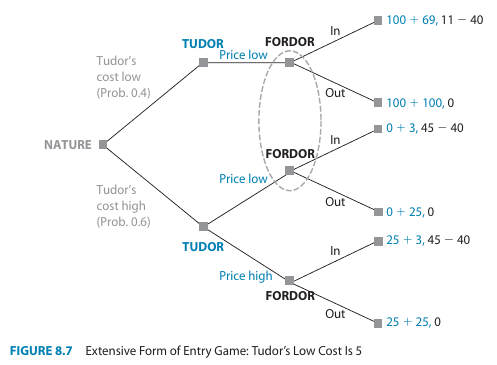
\includegraphics[width=.9\textwidth]{figures/Fig87.png} 
  \end{center} 
\end{frame}

% - - - - - - - - - - - - - - - - - - - - - - - - - - - - - - - - - - - - - - - 

\begin{frame}{Market Entry Game}
  \textbf{Signaling Strategies}
  \begin{itemize}
    \item Tudor might use its price as a \alert{signal} of its cost.
    \item A \textit{low-cost} firm would charge a lower price, 
    so Tudor might hope to keep its price low to show Fordor that they 
    are a low-cost firm and therefore more difficult to fight.
    \item However, Tudor might also try to \textbf{bluff} Fordor 
    into staying out.
  \end{itemize}
\end{frame}

% - - - - - - - - - - - - - - - - - - - - - - - - - - - - - - - - - - - - - - - 

\begin{frame}{Market Entry Game - Separating Equilibrium}
  \textbf{Checking for Separating Equilibrium:} 
  \begin{enumerate}
    \item \textbf{Step 1:} Prune strategies using rollback: 
    \begin{itemize}
      \item What should \alert{Fordor} do if they see a \textbf{high price}?
    \end{itemize}
  \end{enumerate}
  \begin{center}
    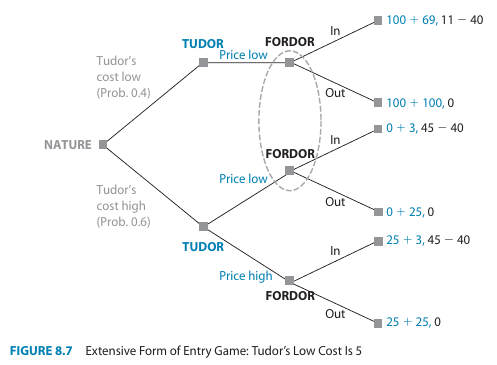
\includegraphics[width=.7\textwidth]{figures/Fig87.png} 
  \end{center} 
\end{frame}

% - - - - - - - - - - - - - - - - - - - - - - - - - - - - - - - - - - - - - - - 

\begin{frame}{Market Entry Game - Separating Equilibrium}
  \textbf{Checking for Separating Equilibrium:} \\ 
  \begin{itemize}
    \item How many Strategies does each player have? 
    \begin{itemize}
      \item (After pruning \textit{Out if Price High} for \alert{Fordor}) 
    \end{itemize}
  \end{itemize}
\end{frame}

% - - - - - - - - - - - - - - - - - - - - - - - - - - - - - - - - - - - - - - - 

\begin{frame}{Market Entry Game - Separating Equilibrium}
  \textbf{Checking for Separating Equilibrium:} \\ 
  \textbf{Step 2:} Represent game in \textit{Strategic Form:}
  \begin{center}
    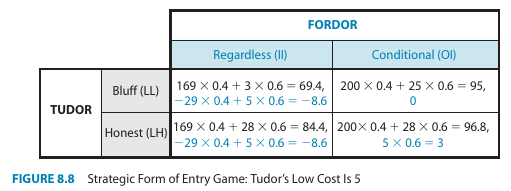
\includegraphics[width =.9\textwidth]{figures/Fig88.png} 
  \end{center}
\end{frame}

% - - - - - - - - - - - - - - - - - - - - - - - - - - - - - - - - - - - - - - - 

\begin{frame}{Market Entry Game - Separating Equilibrium}
  \textbf{Checking for Separating Equilibrium:} \\ 
  \textbf{Step 3:} Look for NE in the \textit{Strategic Form}
  \begin{center}
    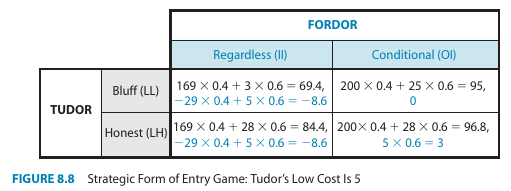
\includegraphics[width =.9\textwidth]{figures/Fig88.png} 
  \end{center}
\end{frame}

% - - - - - - - - - - - - - - - - - - - - - - - - - - - - - - - - - - - - - - - 

\begin{frame}{Market Entry Game - Separating Equilibrium}
  \textbf{Checking for Separating Equilibrium:} \\ 
  \begin{itemize}
    \item So when Tudor's Low Cost is 5, 
    the Nash Equilibrium is (Honest, Conditional)
    \item This is a \textit{Separating} equilibrium,
    because the Tudor's action of \textit{Price High} or \textit{Price Low}
    completely reveals their type to Fordor.
  \end{itemize}
\end{frame}

% - - - - - - - - - - - - - - - - - - - - - - - - - - - - - - - - - - - - - - - 

\begin{frame}{Market Entry Game}
  Is it guaranteed that this game will \textit{always} 
  result in complete separation of types?
  \begin{itemize}
    \item What if we change the Tudor's Low Cost to 10 instead of 5? 
  \end{itemize}
\end{frame}

% - - - - - - - - - - - - - - - - - - - - - - - - - - - - - - - - - - - - - - - 

\begin{frame}{Market Entry Game - Pooling Equilibrium}
  Can you prune any strategies?
  \begin{center}
    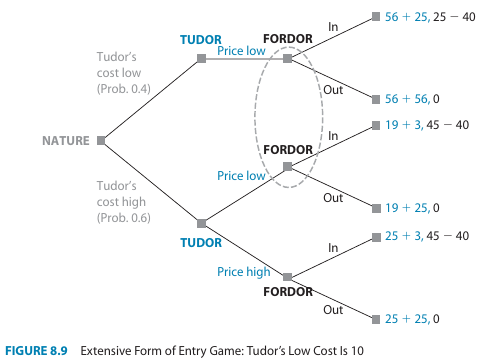
\includegraphics[width=.9\textwidth]{figures/Fig89.png}
  \end{center}
\end{frame}

% - - - - - - - - - - - - - - - - - - - - - - - - - - - - - - - - - - - - - - - 

\begin{frame}{Market Entry Game - Pooling Equilibrium}
  Now what is the Nash Equilibrium of this game?
  \begin{center}
    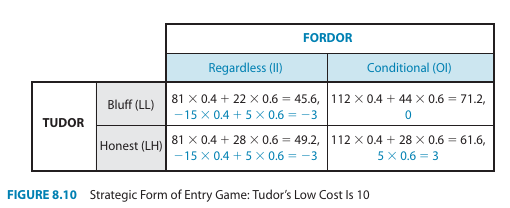
\includegraphics[width=.9\textwidth]{figures/Fig810.png}
  \end{center}
\end{frame}

% - - - - - - - - - - - - - - - - - - - - - - - - - - - - - - - - - - - - - - - 

\begin{frame}{Market Entry Game - Pooling Equilibrium}
  \begin{itemize}
    \item So when Tudor's Low Cost is \alert{10}, 
    the Nash Equilibrium is (\alert{Bluff}, Conditional)
    \item This is a \textit{Pooling} equilibrium,
    because Tudor always takes the same action of \textit{Price Low}. \\ 
    This gives Fordor no signal of their type, 
    but Fordor still doesn't have any incentive to change their strategy.
  \end{itemize}
\end{frame}

% - - - - - - - - - - - - - - - - - - - - - - - - - - - - - - - - - - - - - - - 

\begin{frame}{Market Entry Game}
  \begin{itemize}
    \item So far, we found that depending on the relative difference
    between a \textit{low-cost} Tudor and a \textit{high-cost} Tudor,
    there may either be a \textbf{Pooling} or \textbf{Separating} equilibrium.
    \item But there might also be an equilibrium somewhere in between: 
    where there is \textit{partial} sorting of types
    \item We call this type of equilibrium \textbf{Semiseparating}
  \end{itemize}
\end{frame}

% - - - - - - - - - - - - - - - - - - - - - - - - - - - - - - - - - - - - - - - 

\begin{frame}{Market Entry Game - Semiseparating}
  Now let's change the original probability that a Tudor is low cost
  from .4 to .1
  \begin{itemize}
    \item (But keep all of the payoffs the same as in the last case) 
  \end{itemize}
\end{frame}

% - - - - - - - - - - - - - - - - - - - - - - - - - - - - - - - - - - - - - - - 

\begin{frame}{Market Entry Game - Semiseparating}
  Can you find a Nash Equilibrium with the new expected utilities? 
  \begin{center}
    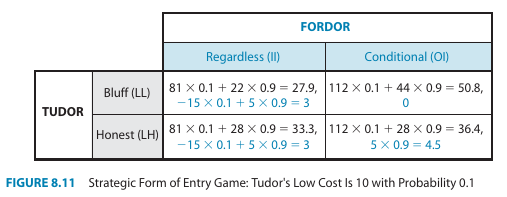
\includegraphics[width=1.0\textwidth]{figures/Fig811.png} 
  \end{center}
\end{frame}

% - - - - - - - - - - - - - - - - - - - - - - - - - - - - - - - - - - - - - - - 

\begin{frame}{Market Entry Game - Semiseparating}
  \textbf{Looking for Mixed Strategy Nash Equilibrium} 
  \begin{itemize}
    \item Suppose \alert{Tudor} plays Bluff with probability $p$,
    Honest with $1-p$ 
    \item When will \alert{Fordor} play a mixed strategy?
  \end{itemize}
\end{frame}

% - - - - - - - - - - - - - - - - - - - - - - - - - - - - - - - - - - - - - - - 

\begin{frame}[plain]{}
  
\end{frame}

% - - - - - - - - - - - - - - - - - - - - - - - - - - - - - - - - - - - - - - - 

\begin{frame}{Market Entry Game - Semiseparating}
  \textbf{Looking for Mixed Strategy Nash Equilibrium} 
  \begin{itemize}
    \item Suppose \alert{Fordor} plays Regardless with probability $q$,
    Conditional with $1-q$ 
    \item When will \alert{Tudor} play a mixed strategy?
  \end{itemize}
\end{frame}

% - - - - - - - - - - - - - - - - - - - - - - - - - - - - - - - - - - - - - - - 

\begin{frame}[plain]{}
  
\end{frame}

% - - - - - - - - - - - - - - - - - - - - - - - - - - - - - - - - - - - - - - - 

\begin{frame}{Market Entry Game - Semiseparating}
  \begin{itemize}
  \item So this version of the game has the MSNE:\\ 
  $\{$ (1/3 Bluff, 2/3 Honest), (16/22 Regardless, 6/22 Conditional) $\}$
  \begin{itemize}
    \item In this equilibrium, instead of \textit{complete separation}  
    or \textit{complete pooling}, 
    we have \alert{\textit{semiseparating}}
    \item A high price conveys full information to Fordor, 
    but a low price could mean that the Tudor is \textit{either} 
    a \textbf{low-price} \textit{or} a \textbf{high-price} type.
  \end{itemize}
  \end{itemize}
\end{frame}

% - - - - - - - - - - - - - - - - - - - - - - - - - - - - - - - - - - - - - - - 

\begin{frame}{Market Entry Game - Semiseparating}
  \textbf{Bayes' Rule} 
  \begin{center}
    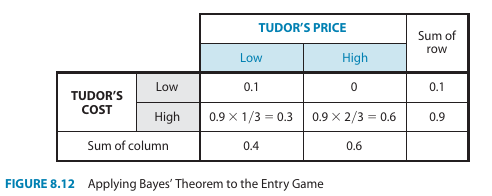
\includegraphics[width=.9\textwidth]{figures/Fig812.png} 
  \end{center}
\end{frame}


% Asymmetric Info example from Silicon Valley 4x02
% - - - - - - - - - - - - - - - - - - - - - - - - - - - - - - - - - - - - - - - 
\begin{frame}{The CEO's new clothes}
  
  \href{https://youtu.be/_1Tn1qqBrhM}{clip}
  
  \alert{Dinesh} has let the power of a CEO position go to his head.
  His new confidence/vanity has led him to trying out a new hairstyle,
  but he starts to suspect that there is a non-zero probability 
  that he looks \textbf{ridiculous} to other people. 

\end{frame}

% - - - - - - - - - - - - - - - - - - - - - - - - - - - - - - - - - - - - - - - 

\begin{frame}{The CEO's new clothes}
  
  Suppose that looking \textbf{ridiculous} is not something that \alert{Dinesh} can 
  subjectively observe about himself, 
  but is only observable by the people around him.
  
  \alert{Gilfoyle} can observe whether or not \alert{Dinesh} looks \textbf{ridiculous}
  and would like it if \alert{Dinesh} embarrassed himself 
  by looking \textbf{ridiculous} in public.

  But he knows that if \alert{Dinesh} thinks he looks \textbf{ridiculous} , 
  he will want to change his look back to the more boring (but less risky)
  style he had as a nerdy programmer. 

\end{frame}

% - - - - - - - - - - - - - - - - - - - - - - - - - - - - - - - - - - - - - - - 

\begin{frame}{The CEO's new clothes}

   Suppose that \alert{Dinesh}'s preferences (from best to worst) are as follows:
  \begin{itemize}
    \item He wears his \textit{new style} proudly and people think he is \textbf{cool}
    \item He wears his \textit{old style} and people think he looks average
    \item He wears his \textit{new style} but people think it is \textbf{ridiculous}
  \end{itemize}
  
  Suppose that \alert{Gilfoyle}'s preferences are:
  \begin{itemize}
    \item \alert{Dinesh} looks \textbf{ridiculous} with the \textit{new style}, 
    continues to wear it and gets embarrassed in public
    \item \alert{Dinesh} goes back to his \textit{old style} 
    \item \alert{Dinesh} looks \textbf{cool} with the \textit{new style},
    continues to wear it and people think he's cool. 
  \end{itemize}
 
\end{frame}

% - - - - - - - - - - - - - - - - - - - - - - - - - - - - - - - - - - - - - - - 

\begin{frame}{The CEO's new clothes}
  Model this as an asymmetric information game 
  where \alert{Gilfoyle} has the private information 
  of whether \alert{Dinesh} looks \textbf{ridiculous}.
  \vspace{60mm}
\end{frame}

% - - - - - - - - - - - - - - - - - - - - - - - - - - - - - - - - - - - - - - - 

\begin{frame}{}
  
\end{frame}


\end{document}
